% Orleans.GpuBridge Executive Overview
% Compile with: pdflatex gpubridge-executive-overview.tex (run twice for TOC)
\documentclass[11pt,a4paper]{article}

% ── Packages ──────────────────────────────────────────────────────────────────
\usepackage[utf8]{inputenc}
\usepackage[T1]{fontenc}
\usepackage{lmodern}
\usepackage[margin=2.4cm]{geometry}
\usepackage{graphicx}
\usepackage{xcolor}
\usepackage{titlesec}
\usepackage{enumitem}
\usepackage{booktabs}
\usepackage{tabularx}
\usepackage{multirow}
\usepackage{fancyhdr}
\usepackage{hyperref}
\usepackage{amssymb}
\usepackage{tcolorbox}
\usepackage{needspace}
\usepackage{tikz}
\usetikzlibrary{arrows.meta, positioning, calc, shapes.geometric}

% ── Colours ───────────────────────────────────────────────────────────────────
\definecolor{brand}{HTML}{1A2744}      % Deep navy
\definecolor{accent}{HTML}{E67E22}     % Warm orange
\definecolor{highlight}{HTML}{D35400}  % Deep orange
\definecolor{success}{HTML}{2D936C}    % Green
\definecolor{lightbg}{HTML}{FDF6EF}    % Warm light background
\definecolor{midgray}{HTML}{6C757D}    % Muted text

% ── Heading styles ────────────────────────────────────────────────────────────
\titleformat{\section}
  {\Large\bfseries\color{brand}}
  {\thesection}{1em}{}[\vspace{-0.4em}\textcolor{accent}{\rule{\textwidth}{1.2pt}}]

\titleformat{\subsection}
  {\large\bfseries\color{brand}}
  {\thesubsection}{0.8em}{}

\titleformat{\subsubsection}
  {\normalsize\bfseries\color{accent}}
  {\thesubsubsection}{0.6em}{}

% ── Header / Footer ──────────────────────────────────────────────────────────
\pagestyle{fancy}
\fancyhf{}
\renewcommand{\headrulewidth}{0.4pt}
\fancyhead[L]{\small\textcolor{midgray}{Orleans.GpuBridge --- Executive Overview}}
\fancyhead[R]{\small\textcolor{midgray}{v0.2.1}}
\fancyfoot[C]{\small\textcolor{midgray}{\thepage}}

% ── Custom boxes ──────────────────────────────────────────────────────────────
\tcbset{
  keybox/.style={
    colback=lightbg, colframe=accent, boxrule=0.6pt,
    arc=3pt, left=8pt, right=8pt, top=6pt, bottom=6pt,
    colbacktitle=accent, coltitle=white,
    fonttitle=\bfseries, title=#1
  },
  statbox/.style={
    colback=white, colframe=brand, boxrule=0.8pt,
    arc=4pt, left=6pt, right=6pt, top=4pt, bottom=4pt,
    width=0.30\textwidth
  }
}

% ── Hyperref setup ────────────────────────────────────────────────────────────
\hypersetup{
  colorlinks=true,
  linkcolor=brand,
  urlcolor=accent,
  citecolor=brand,
  pdftitle={Orleans.GpuBridge -- GPU-Native Distributed Computing for Orleans},
  pdfauthor={Michael Ivertowski},
  pdfsubject={Executive Overview},
}

% ══════════════════════════════════════════════════════════════════════════════
\begin{document}

% ── Title page ────────────────────────────────────────────────────────────────
\begin{titlepage}
\begin{tikzpicture}[remember picture, overlay]
  % Background gradient bar
  \fill[brand] (current page.north west) rectangle
    ([yshift=-9cm]current page.north east);
  % Accent stripe
  \fill[accent] ([yshift=-9cm]current page.north west) rectangle
    ([yshift=-9.4cm]current page.north east);
  % Decorative dots
  \foreach \x in {0.5,1.0,...,5.0} {
    \foreach \y in {0.5,1.0,...,3.0} {
      \fill[white, opacity=0.04] ([xshift=\x cm, yshift=-\y cm]current page.north west)
        circle (1.5pt);
    }
  }
\end{tikzpicture}

\vspace*{1.5cm}
\begin{flushleft}
  {\fontsize{34}{40}\selectfont\bfseries\textcolor{white}{Orleans.GpuBridge}}\\[0.5em]
  {\fontsize{16}{20}\selectfont\textcolor{white!85}{GPU-Native Distributed Computing for Orleans}}\\[0.3em]
  {\large\textcolor{white!65}{Sub-Microsecond Actor Messaging on GPU Hardware}}\\[0.3em]
  {\normalsize\textcolor{white!50}{.NET 9 \textbullet{} Ring Kernels \textbullet{} Temporal Alignment \textbullet{} DotCompute Backend}}
\end{flushleft}

\vspace{5.5cm}

\begin{flushleft}
  \textcolor{midgray}{\large Executive Overview}\\[0.8em]
  {\Large\textcolor{brand}{\textbf{Version 0.2.1}}}\\[1.5em]
  \textcolor{midgray}{%
    A paradigm shift from CPU-based actor systems to actors that\\
    live permanently on the GPU --- achieving 100--500\,ns message\\
    latency and 2\,M messages/second throughput.%
  }
\end{flushleft}

\vfill
\begin{flushleft}
  \textcolor{midgray}{\small
    Built with .NET 9 \& C\# \textbullet{} 11 modular packages \textbullet{} 1,200+ tests\\[4pt]
    Open-source (Apache-2.0) \textbullet{} Commercial license available\\[4pt]
    \textbf{Contact:} \href{mailto:michael.ivertowski@ch.ey.com}{michael.ivertowski@ch.ey.com}
  }
\end{flushleft}
\end{titlepage}

% ── Table of Contents ─────────────────────────────────────────────────────────
\tableofcontents
\newpage

% ══════════════════════════════════════════════════════════════════════════════
\section{Executive Summary}

Orleans.GpuBridge is a .NET~9 library that enables GPU-native distributed
computing for Microsoft Orleans. Rather than treating the GPU as an
accelerator to which work is occasionally dispatched, it introduces a
fundamentally new model: \emph{actors that reside permanently in GPU memory},
communicating through lock-free ring-buffer message queues at hardware speed.

The result is a 20--200$\times$ improvement over traditional CPU-based actor
systems, with message latencies of 100--500\,ns on datacenter GPUs and
throughput exceeding 2\,M~messages/second per actor.

\begin{tcolorbox}[keybox={Why Orleans.GpuBridge?}]
\begin{itemize}[leftmargin=1.2em, itemsep=3pt]
  \item \textbf{GPU-native actors} --- actors live permanently in GPU memory;
        zero kernel-launch overhead eliminates the dominant cost of
        traditional GPU offloading.
  \item \textbf{Ring kernels} --- persistent GPU kernels running infinite
        dispatch loops process messages without repeated launch cycles.
  \item \textbf{Temporal alignment} --- Hybrid Logical Clocks and Vector
        Clocks execute \emph{on the GPU}, providing causal ordering at
        hardware speed.
  \item \textbf{Familiar .NET patterns} --- standard \texttt{async/await}
        C\# programming model with automatic CPU fallback when no GPU is
        available.
  \item \textbf{Production-grade resilience} --- Polly~v8 integration with
        circuit breakers, rate limiting, retry policies, and comprehensive
        health checks.
  \item \textbf{Cross-platform GPU support} --- CUDA, OpenCL, DirectCompute,
        and Metal through the DotCompute abstraction layer.
\end{itemize}
\end{tcolorbox}

\subsection{At a Glance}

\vspace{0.6em}
\begin{center}
\begin{tabular}{@{}c@{\hspace{1.8em}}c@{\hspace{1.8em}}c@{}}
\begin{tcolorbox}[statbox, width=4.8cm]
  \centering
  {\fontsize{26}{30}\selectfont\bfseries\textcolor{accent}{100--500\,ns}}\\[3pt]
  {\small message latency (datacenter GPU)}
\end{tcolorbox} &
\begin{tcolorbox}[statbox, width=4.8cm]
  \centering
  {\fontsize{26}{30}\selectfont\bfseries\textcolor{accent}{2\,M+}}\\[3pt]
  {\small messages/sec per actor}
\end{tcolorbox} &
\begin{tcolorbox}[statbox, width=4.8cm]
  \centering
  {\fontsize{26}{30}\selectfont\bfseries\textcolor{accent}{20--200$\times$}}\\[3pt]
  {\small faster than CPU actors}
\end{tcolorbox}
\end{tabular}
\end{center}

% ══════════════════════════════════════════════════════════════════════════════
\section{The GPU-Native Paradigm}

\subsection{Traditional vs.\ GPU-Native Actors}

The conventional approach treats the GPU as a coprocessor: CPU actors
serialize data, launch a kernel, wait for completion, and deserialize
results. Each dispatch incurs 10--50\,$\mu$s of launch overhead.

Orleans.GpuBridge eliminates this entirely. Actors are allocated in GPU
memory and communicate through lock-free ring-buffer queues. A persistent
\emph{ring kernel} runs an infinite dispatch loop, routing messages to
actors without ever returning to the CPU.

\begin{center}
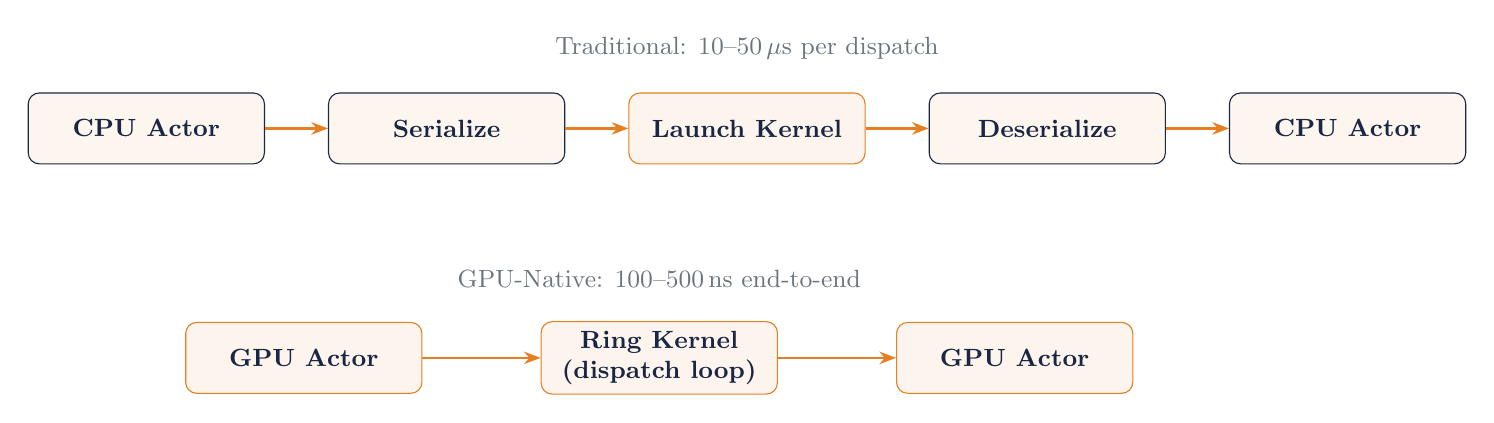
\begin{tikzpicture}[
  node distance=0.8cm,
  box/.style={draw=brand, fill=lightbg, rounded corners=4pt,
              minimum width=3.0cm, minimum height=0.9cm,
              font=\small\bfseries, text=brand, align=center},
  gpubox/.style={draw=accent, fill=accent!8, rounded corners=4pt,
              minimum width=3.0cm, minimum height=0.9cm,
              font=\small\bfseries, text=brand, align=center},
  arr/.style={-{Stealth[length=6pt]}, thick, color=accent}
]
  % Traditional
  \node[box] (cpu1) {CPU Actor};
  \node[box, right=of cpu1] (ser) {Serialize};
  \node[gpubox, right=of ser] (kernel) {Launch Kernel};
  \node[box, right=of kernel] (deser) {Deserialize};
  \node[box, right=of deser] (cpu2) {CPU Actor};

  \draw[arr] (cpu1) -- (ser);
  \draw[arr] (ser) -- (kernel);
  \draw[arr] (kernel) -- (deser);
  \draw[arr] (deser) -- (cpu2);

  \node[above=0.3cm of kernel, font=\small\color{midgray}]
    {Traditional: 10--50\,$\mu$s per dispatch};

  % GPU-Native
  \node[gpubox, below=2.0cm of cpu1, xshift=2.0cm] (ga1) {GPU Actor};
  \node[gpubox, right=1.5cm of ga1] (ring) {Ring Kernel\\(dispatch loop)};
  \node[gpubox, right=1.5cm of ring] (ga2) {GPU Actor};

  \draw[arr] (ga1) -- (ring);
  \draw[arr] (ring) -- (ga2);

  \node[above=0.3cm of ring, font=\small\color{midgray}]
    {GPU-Native: 100--500\,ns end-to-end};
\end{tikzpicture}
\end{center}

\subsection{Performance Comparison}

\vspace{0.5em}
\noindent
\renewcommand{\arraystretch}{1.2}
\begin{tabularx}{\textwidth}{>{\bfseries\color{brand}}l c c c}
\toprule
\textbf{Metric} & \textbf{CPU Actors} & \textbf{GPU Offload} & \textbf{GPU-Native} \\
\midrule
Message Latency     & 10--100\,$\mu$s & 10--50\,$\mu$s & 100--500\,ns \\
Throughput          & 15\,K msg/s     & 50\,K msg/s    & 2\,M msg/s \\
Memory Bandwidth    & 200\,GB/s       & 500\,GB/s      & 1,935\,GB/s \\
Kernel Overhead     & N/A             & 10--50\,$\mu$s  & 0 (persistent) \\
Improvement         & ---             & 2--5$\times$    & \textbf{20--200$\times$} \\
\bottomrule
\end{tabularx}
\vspace{0.5em}

% ══════════════════════════════════════════════════════════════════════════════
\section{Core Technology}

\subsection{Ring Kernel Infrastructure}

Ring kernels are persistent GPU kernels that never terminate. Each kernel
runs an infinite dispatch loop, polling a lock-free message queue and
routing messages to GPU-resident actors. This architecture delivers three
key properties:

\begin{enumerate}[leftmargin=1.4em, itemsep=3pt]
  \item \textbf{Zero launch overhead} --- the kernel is always running;
        no CUDA \texttt{cudaLaunchKernel} calls are needed per message.
  \item \textbf{GPU-resident state} --- actor state lives in GPU global
        memory, eliminating PCIe transfer costs.
  \item \textbf{Hardware-speed messaging} --- messages traverse GPU shared
        memory at DRAM bandwidth ($>$1\,TB/s on modern GPUs).
\end{enumerate}

\subsection{Temporal Alignment}

Distributed actor systems require causal ordering of events.
Orleans.GpuBridge implements two complementary clock mechanisms
\emph{directly on the GPU}:

\vspace{0.5em}
\noindent
\renewcommand{\arraystretch}{1.2}
\begin{tabularx}{\textwidth}{>{\bfseries\color{brand}}l X}
\toprule
\textbf{Mechanism} & \textbf{Description} \\
\midrule
Hybrid Logical Clock &
  Combines physical wall-clock time with a logical counter to provide
  globally ordered timestamps without synchronization barriers. \\
Vector Clocks &
  Per-actor logical clocks that capture causal ``happens-before''
  relationships, enabling precise conflict detection in concurrent
  GPU operations. \\
Latency Compensator &
  Adaptive calibration using exponentially weighted moving averages
  to compensate for inter-node clock skew in multi-silo deployments. \\
\bottomrule
\end{tabularx}
\vspace{0.5em}

\subsection{GPU-to-GPU Direct Messaging}

Actors on different GPUs communicate through a peer-to-peer messaging
layer that avoids CPU round-trips. When NVLink or peer-to-peer PCIe access
is available, messages bypass the CPU entirely. On systems without P2P
support, the framework automatically falls back to CPU-mediated transfers
with no API changes required.

% ══════════════════════════════════════════════════════════════════════════════
\section{Architecture}

\subsection{Package Structure}

Orleans.GpuBridge is organized as eleven modular NuGet packages, each with
a clear responsibility boundary:

\begin{center}
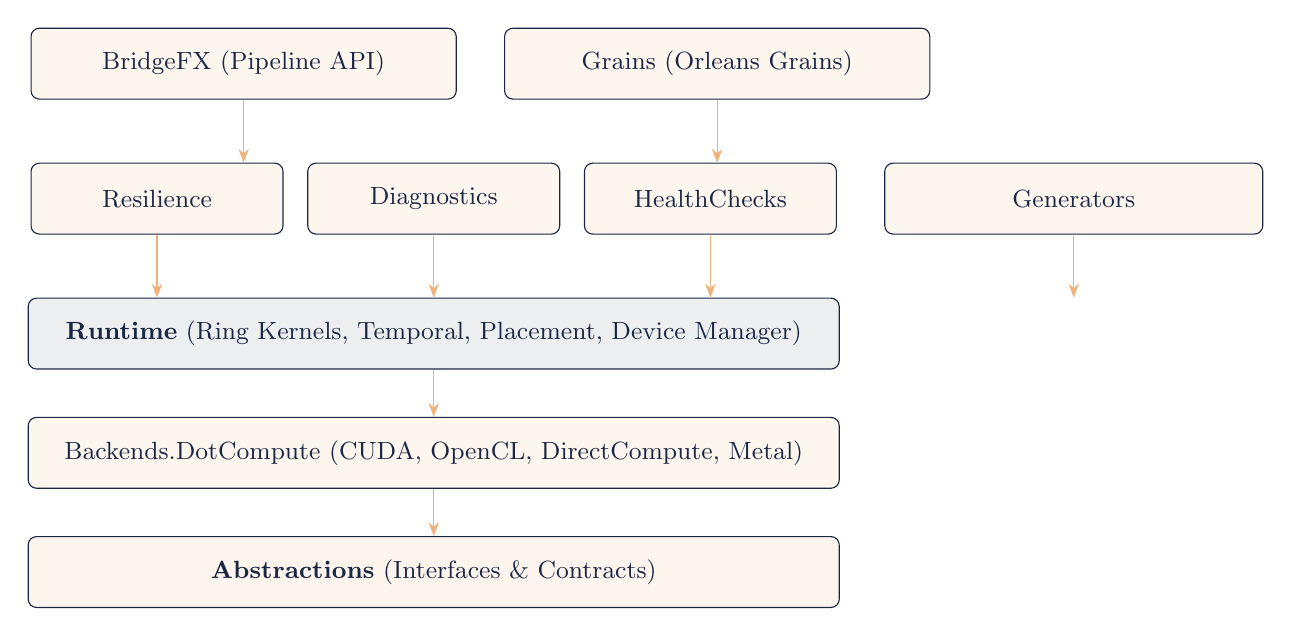
\begin{tikzpicture}[
  node distance=0.5cm,
  layer/.style={draw=brand, fill=lightbg, rounded corners=3pt,
                minimum height=0.9cm, font=\small, text=brand, align=center},
  arr/.style={-{Stealth[length=5pt]}, color=accent!60}
]
  % Top layer
  \node[layer, minimum width=5.4cm] (bridgefx) {BridgeFX (Pipeline API)};
  \node[layer, minimum width=5.4cm, right=0.6cm of bridgefx] (grains) {Grains (Orleans Grains)};

  % Middleware layer
  \node[layer, minimum width=3.2cm, below=0.8cm of bridgefx.south west,
        anchor=north west] (resilience) {Resilience};
  \node[layer, minimum width=3.2cm, right=0.3cm of resilience] (diagnostics) {Diagnostics};
  \node[layer, minimum width=3.2cm, right=0.3cm of diagnostics] (health) {HealthChecks};

  % Runtime
  \node[layer, minimum width=10.3cm, below=0.8cm of diagnostics, fill=brand!8]
    (runtime) {\textbf{Runtime} (Ring Kernels, Temporal, Placement, Device Manager)};

  % Backend
  \node[layer, minimum width=10.3cm, below=0.6cm of runtime]
    (dotcompute) {Backends.DotCompute (CUDA, OpenCL, DirectCompute, Metal)};

  % Abstractions
  \node[layer, minimum width=10.3cm, below=0.6cm of dotcompute, fill=accent!8]
    (abstractions) {\textbf{Abstractions} (Interfaces \& Contracts)};

  % Supporting
  \node[layer, minimum width=4.8cm, right=0.6cm of health] (generators) {Generators};

  % Arrows
  \draw[arr] (bridgefx.south) -- (bridgefx.south |- resilience.north);
  \draw[arr] (grains.south) -- (grains.south |- health.north);

  \draw[arr] (resilience.south) -- (resilience.south |- runtime.north);
  \draw[arr] (diagnostics.south) -- (runtime.north);
  \draw[arr] (health.south) -- (health.south |- runtime.north);
  \draw[arr] (generators.south) -- (generators.south |- runtime.north);

  \draw[arr] (runtime.south) -- (dotcompute.north);
  \draw[arr] (dotcompute.south) -- (abstractions.north);
\end{tikzpicture}
\end{center}

\needspace{8\baselineskip}
\subsection{Key Packages}

\vspace{0.5em}
\noindent
\renewcommand{\arraystretch}{1.2}
\begin{tabularx}{\textwidth}{>{\bfseries\color{brand}}l X}
\toprule
\textbf{Package} & \textbf{Responsibility} \\
\midrule
Abstractions &
  Core interfaces: \texttt{IGpuDevice}, \texttt{IGpuKernel},
  \texttt{IGpuBuffer}, \texttt{IRingKernelRuntime}, temporal contracts. \\
Runtime &
  Ring kernel management, device discovery, queue-depth placement,
  adaptive load balancing, HLC/Vector Clock implementation. \\
Grains &
  Orleans grain base classes: \texttt{GpuGrainBase},
  \texttt{RingKernelGrainBase} with lifecycle integration. \\
BridgeFX &
  High-level fluent API for GPU pipeline construction with
  \texttt{async/await} support. \\
Backends.DotCompute &
  Cross-platform GPU backend via DotCompute --- CUDA, OpenCL,
  DirectCompute, and Metal. \\
Resilience &
  Polly~v8 policies: circuit breaker, retry, timeout, rate limiting,
  and bulkhead isolation. \\
Diagnostics &
  OpenTelemetry metrics, GPU memory telemetry, structured logging. \\
HealthChecks &
  ASP.NET Core health checks for GPU device status and kernel liveness. \\
Generators &
  Compile-time source generators for GPU actor boilerplate. \\
\bottomrule
\end{tabularx}
\vspace{0.5em}

% ══════════════════════════════════════════════════════════════════════════════
\newpage
\section{Advanced Features}

\subsection{Hypergraph Actors}

Traditional actor graphs model pairwise relationships. Orleans.GpuBridge
introduces \emph{hypergraph actors} that represent multi-way relationships
--- a single hyperedge can connect three or more actors simultaneously.

\begin{tcolorbox}[keybox={Hypergraph Advantages}]
\begin{itemize}[leftmargin=1.2em, itemsep=3pt]
  \item \textbf{Pattern matching} --- GPU-accelerated subgraph isomorphism
        at 10--500$\times$ the speed of CPU implementations.
  \item \textbf{Multi-party transactions} --- model complex business events
        involving multiple entities without decomposing into pairwise edges.
  \item \textbf{Temporal hyperedges} --- each relationship carries HLC
        timestamps for causal ordering and temporal queries.
  \item \textbf{Dynamic topology} --- actors can join/leave hyperedges at
        runtime without global coordination.
\end{itemize}
\end{tcolorbox}

\needspace{8\baselineskip}
\subsection{Adaptive Placement \& Load Balancing}

Orleans.GpuBridge extends Orleans' placement model with GPU-aware strategies:

\vspace{0.5em}
\noindent
\renewcommand{\arraystretch}{1.2}
\begin{tabularx}{\textwidth}{>{\bfseries\color{brand}}l X}
\toprule
\textbf{Strategy} & \textbf{Behaviour} \\
\midrule
Queue-Depth Placement &
  Routes grain activations to the GPU with the shortest message queue,
  minimizing tail latency. \\
Adaptive Load Balancer &
  Continuously monitors GPU utilization, memory pressure, and thermal
  state; rebalances actors across devices when thresholds are exceeded. \\
Memory-Aware Eviction &
  When GPU memory is constrained, cold actors are transparently migrated
  to CPU with automatic re-promotion on next access. \\
\bottomrule
\end{tabularx}
\vspace{0.5em}

\subsection{Resilience Patterns}

Built on Polly~v8, the resilience layer provides production-grade fault
tolerance:

\begin{itemize}[leftmargin=1.4em, itemsep=2pt]
  \item \textbf{Circuit breaker} --- halts GPU dispatch after configurable
        failure thresholds; auto-recovers after a cooling period.
  \item \textbf{Retry with backoff} --- exponential and jittered retry for
        transient GPU errors (driver timeouts, memory allocation failures).
  \item \textbf{Rate limiting} --- token-bucket rate limiter prevents GPU
        overload during burst traffic.
  \item \textbf{Timeout management} --- per-kernel and per-pipeline timeouts
        with graceful cancellation via \texttt{CancellationToken}.
  \item \textbf{Bulkhead isolation} --- limits concurrent GPU operations to
        prevent resource starvation.
\end{itemize}

% ══════════════════════════════════════════════════════════════════════════════
\section{GPU Platform Support}

\subsection{Backend Matrix}

Orleans.GpuBridge supports five GPU compute backends through the DotCompute
abstraction layer. A unified API surface ensures application code is
backend-agnostic.

\vspace{0.5em}
\noindent
\renewcommand{\arraystretch}{1.2}
\begin{tabularx}{\textwidth}{>{\bfseries\color{brand}}l c c c X}
\toprule
\textbf{Backend} & \textbf{Windows} & \textbf{Linux} & \textbf{macOS} & \textbf{Notes} \\
\midrule
CUDA          & \checkmark & \checkmark & ---        & NVIDIA GPUs; full ring kernel support \\
OpenCL        & \checkmark & \checkmark & \checkmark & Multi-vendor; broadest hardware reach \\
DirectCompute & \checkmark & ---        & ---        & DirectX 11+ integrated workloads \\
Metal         & ---        & ---        & \checkmark & Apple Silicon native compute \\
Vulkan        & \multicolumn{3}{c}{\textit{planned}} & Cross-vendor next-gen API \\
\bottomrule
\end{tabularx}
\vspace{0.5em}

\subsection{GPU Hardware Tiers}

The ring kernel execution model adapts to the coherence capabilities of
the target GPU:

\vspace{0.5em}
\noindent
\renewcommand{\arraystretch}{1.2}
\begin{tabularx}{\textwidth}{>{\bfseries\color{brand}}l l l X}
\toprule
\textbf{Tier} & \textbf{Mode} & \textbf{Latency} & \textbf{Hardware Examples} \\
\midrule
Full Coherence &
  Persistent kernel &
  100--500\,ns &
  A100, H100, Grace Hopper \\
Partial Coherence &
  EventDriven &
  1--10\,ms &
  RTX 2000/3000/4000 series \\
Limited &
  EventDriven &
  $\sim$5\,s &
  WSL2 environments; development only \\
\bottomrule
\end{tabularx}
\vspace{0.5em}

\noindent
On hardware without GPU coherence, the framework transparently falls back
to EventDriven mode --- the same API, different dispatch strategy, no code
changes required.

% ══════════════════════════════════════════════════════════════════════════════
\section{Deployment Models}

Orleans.GpuBridge supports two deployment models that coexist in the same
Orleans silo. Developers choose per-grain which model to use, and the
framework handles resource allocation, fallback, and lifecycle management.

\vspace{0.5em}
\noindent
\renewcommand{\arraystretch}{1.2}
\begin{tabularx}{\textwidth}{>{\bfseries\color{brand}}l l X}
\toprule
\textbf{Model} & \textbf{Throughput} & \textbf{Best For} \\
\midrule
GPU-Offload &
  15\,K msg/s &
  Batch processing, infrequent GPU usage ($<$10 calls/sec).
  CPU actors dispatch kernels to GPU on demand. \\
GPU-Native &
  2\,M msg/s &
  High-frequency messaging ($>$1\,K msg/s), real-time analytics.
  Actors live permanently in GPU memory with ring kernels. \\
\bottomrule
\end{tabularx}
\vspace{0.5em}

% ══════════════════════════════════════════════════════════════════════════════
\section{Use Cases}

\begin{tcolorbox}[keybox={Primary Use Cases}]
\begin{description}[leftmargin=1em, labelwidth=1em, font=\color{brand}\bfseries]
  \item[$\blacktriangleright$] \textbf{High-Frequency Trading} ---
    Order matching and risk computation at $<$10\,$\mu$s with GPU-resident
    market data and temporal causal ordering.

  \item[$\blacktriangleright$] \textbf{Real-Time Fraud Detection} ---
    Hypergraph pattern matching across transaction networks with
    sub-millisecond anomaly detection.

  \item[$\blacktriangleright$] \textbf{Digital Twins} ---
    Physics-accurate simulation with GPU-native actors representing
    sensors, actuators, and control systems at hardware speed.

  \item[$\blacktriangleright$] \textbf{Process Intelligence} ---
    Object-Centric Process Mining with 640$\times$ speedup for process
    discovery, conformance checking at 450\,$\mu$s.

  \item[$\blacktriangleright$] \textbf{Stream Processing} ---
    GPU-accelerated event stream analytics with $<$100\,$\mu$s end-to-end
    latency for IoT, telemetry, and log analysis.

  \item[$\blacktriangleright$] \textbf{Scientific Computing} ---
    Molecular dynamics, particle systems, and genome alignment using
    the familiar Orleans actor model with GPU acceleration.

  \item[$\blacktriangleright$] \textbf{Graph Analytics} ---
    Temporal hypergraph queries, centrality computation, and community
    detection at GPU memory bandwidth.
\end{description}
\end{tcolorbox}

% ══════════════════════════════════════════════════════════════════════════════
\newpage
\section{Quality \& Maturity}

\subsection{Test Coverage}

The project includes \textbf{1,153 automated tests} across 11 test suites,
with \textbf{1,133 passing} and 18 skipped (all with documented reasons:
GPU hardware requirements, full Orleans silo infrastructure, or lock-free
data structure work-in-progress).

\vspace{0.5em}
\noindent
\renewcommand{\arraystretch}{1.15}
\begin{tabularx}{\textwidth}{>{\color{brand}}l r@{\hspace{2em}}l r}
\toprule
\textbf{Test Project} & \textbf{Total} & \textbf{Test Project} & \textbf{Total} \\
\midrule
Abstractions.Tests        & 242 & Hardware.Tests              &  37 \\
Runtime.Tests             & 206 & Backends.DotCompute.Tests   &  56 \\
Temporal.Tests            & 292 & RingKernelTests             &  92 \\
Grains.Tests              &  98 & Performance.Tests           &  20 \\
Generators.Tests          &  22 & Integration.Tests           &  35 \\
                          &     & Resilience.Tests            &  53 \\
\bottomrule
\end{tabularx}
\vspace{0.5em}

\needspace{6\baselineskip}
\subsection{Implementation Status}

\vspace{0.5em}
\noindent
\renewcommand{\arraystretch}{1.15}
\begin{tabularx}{\textwidth}{>{\color{brand}}c l X}
\toprule
& \textbf{Feature} & \textbf{Details} \\
\midrule
\checkmark & Ring kernel infrastructure      & Persistent dispatch loops, message routing \\
\checkmark & GPU-resident message queues      & Lock-free ring buffers in GPU memory \\
\checkmark & Temporal alignment               & HLC \& Vector Clocks on GPU \\
\checkmark & Hypergraph actors                & Multi-way relationships, pattern matching \\
\checkmark & Queue-depth placement            & GPU-aware grain activation routing \\
\checkmark & Adaptive load balancing          & Dynamic rebalancing across devices \\
\checkmark & Resilience (Polly v8)            & Circuit breaker, retry, rate limiting \\
\checkmark & GPU Direct Messaging             & P2P with automatic fallback \\
\checkmark & GPU Memory Telemetry             & Per-grain OpenTelemetry metrics \\
\checkmark & DotCompute backend               & EventDriven mode production-ready \\
$\circ$    & Persistent ring kernel mode      & Requires full GPU coherence hardware \\
$\circ$    & Vulkan compute backend           & Cross-vendor next-gen API \\
$\circ$    & GPUDirect Storage                & NVMe-to-GPU direct path \\
\bottomrule
\end{tabularx}
\vspace{0.5em}

% ══════════════════════════════════════════════════════════════════════════════
\needspace{6\baselineskip}
\section{Getting Started}

\subsection{Installation}

\begin{tcolorbox}[colback=brand!3, colframe=brand!40, boxrule=0.5pt, arc=3pt,
                   left=8pt, right=8pt, top=6pt, bottom=6pt]
\ttfamily\small
\# Add core packages\\
dotnet add package Orleans.GpuBridge.Abstractions\\
dotnet add package Orleans.GpuBridge.Runtime\\
dotnet add package Orleans.GpuBridge.Grains\\[6pt]
\# Add resilience and diagnostics\\
dotnet add package Orleans.GpuBridge.Resilience\\
dotnet add package Orleans.GpuBridge.Diagnostics\\
dotnet add package Orleans.GpuBridge.HealthChecks
\end{tcolorbox}

\subsection{Basic GPU Grain}

\begin{tcolorbox}[colback=brand!3, colframe=brand!40, boxrule=0.5pt, arc=3pt,
                   left=8pt, right=8pt, top=6pt, bottom=6pt]
\ttfamily\small
public class MyGpuGrain : GpuGrainBase, IMyGpuGrain\\
\{\\
\hspace*{1em}public async Task<float[]> ComputeAsync(float[] input)\\
\hspace*{1em}\{\\
\hspace*{2em}using var buffer = await GpuDevice.AllocateAsync(input);\\
\hspace*{2em}await GpuDevice.DispatchAsync("my\_kernel", buffer);\\
\hspace*{2em}return await buffer.ReadAsync();\\
\hspace*{1em}\}\\
\}
\end{tcolorbox}

\subsection{Build \& Test}

\begin{tcolorbox}[colback=brand!3, colframe=brand!40, boxrule=0.5pt, arc=3pt,
                   left=8pt, right=8pt, top=6pt, bottom=6pt]
\ttfamily\small
\# Build the solution\\
dotnet build\\[6pt]
\# Run all tests\\
dotnet test\\[6pt]
\# Build release with NuGet packages\\
dotnet pack -c Release
\end{tcolorbox}

% ══════════════════════════════════════════════════════════════════════════════
\section{Links \& Resources}

\begin{tcolorbox}[keybox={Repository \textnormal{and} Ecosystem}]
\renewcommand{\arraystretch}{1.4}
\begin{tabularx}{\textwidth}{>{\bfseries\color{brand}}l X}
  Repository &
    \url{https://github.com/mivertowski/Orleans.GpuBridge.Core} \\
  Documentation &
    \texttt{docs/} directory --- architecture overviews, API reference,
    article series on GPU-native actors, hypergraph actors, and temporal
    correctness. \\
  NuGet &
    \texttt{Orleans.GpuBridge.*} packages (Abstractions, Runtime, Grains,
    BridgeFX, Resilience, Diagnostics, HealthChecks, Generators) \\
  License &
    Apache-2.0 (open-source); commercial license available \\
\midrule
  Microsoft Orleans &
    Distributed actor framework --- virtual actors, cluster management,
    and grain lifecycle; the foundation this library extends. \\
  DotCompute &
    .NET-native GPU compute abstraction unifying CUDA, OpenCL,
    DirectCompute, and Metal under a single API. \\
  DataSynth &
    Enterprise synthetic data platform for GPU-accelerated analytics. \\
  AssureTwin &
    Native audit intelligence platform using GpuBridge for
    GPU-accelerated graph analytics and process mining. \\
\end{tabularx}
\end{tcolorbox}

\vfill
\begin{center}
\textcolor{midgray}{\rule{0.5\textwidth}{0.4pt}}\\[0.8em]
{\small\textcolor{midgray}{%
  Orleans.GpuBridge v0.2.1 \textbullet{}
  Open-source (Apache-2.0) \textbullet{}
  Commercial license available%
}}\\[4pt]
{\small\textcolor{midgray}{%
  \textbf{Contact:} \href{mailto:michael.ivertowski@ch.ey.com}{michael.ivertowski@ch.ey.com}%
}}
\end{center}

\end{document}
